\chapter{Background}

%intro to the background section here

Although this dissertation discusses a wide variety of work, it all draws on a common foundation. This chapter will lay out that foundation before moving on to discuss specific projects. There are three components to this foundation: design as a research practice, methodology, and related work. I will cover these in order.




% : virtual worlds, face-to-face panel discussions, small group seminar discussions, business meetings, remote information sessions, and live-event spectating

% Part of what's attractive about mediated communication systems is that there is a tremendous variety of ways to design and use them once we set aside a desire to recreate face-to-face interaction. Although in this section I've contrasted mediated communication with face-to-face communication in a way that might imply that mediated communication systems are somehow monolithic and self-similar, the survey of related systems in the section to follow will illustrate the tremendous range of potential systems in this space and demonstrate how thoughtful designs can have widely varying impacts on the experience of communication or collaboration. 

% My work takes this general design strategy of adding new communication channels in a few different directions. In this proposal, I will describe my past work looking at meetings in virtual worlds, audience-speaker interaction in presentations, and classroom discussions. I will also lay out my design for a system to support face-to-face meetings with remote participants. These research contexts vary both in the numbers of simultaneous participants, as well as their geographic configuration. Over the course of my work, I have shifted my attention from configurations where all users are remote (\emph{Information Spaces}) to heterogeneous situations where some or all of the participants are co-located (\emph{backchan.nl}, \emph{Tin Can Classroom}, \emph{Tin Can Conference}). 

% TODO Add a paragraph here that preludes some of the design as research ideas (which will be covered in more depth in their own section) as a way of saying that having these themes is part of what makes this research-worthy. 

\section{Design as Research}

Proposing a design space and arguing for its value as an approach to common problems is not, traditionally, the realm of academic research. It is a frequently taken-for-granted assumption at the Media Lab that designing novel technical systems is a natural and defensible way to do research, but outside of that context this approach is rarely accepted without argument. Given that this assumption is fundamental to my work, it seems useful to address this epistemological question from the start.

Design as research is clearly being conducted in a variety of contexts using a variety of methods, yet there is very little discussion or agreement about the fundamental aspects of how that work is conducted and what we can learn from it. Traditionally it is tolerated, provided that the primary argument for its contribution to the wider discourse is based on a justification from another research field. In computer science related fields, efficiency and technical complexity are reliable ways to argue for the quality of work, even work like mine where novel systems and interactions are described. This has a warping effect on the sorts of systems that are built and studied because there needs to either be a technical challenge in the solution or a way to easily judge the efficiency of the solution relative to existing methods.

Although there are ways to frame my work in those terms, I do not view those as particularly effective ways to judge my work. Instead, in this section I would like to make a positive argument for why building and testing systems may be the \emph{best} approach for certain kinds of research questions. I will describe the sorts of contributions one can make working this way and contrast this approach with other approaches dominant in the fields of human computer interaction, computer mediated communication, and computer supported cooperative work.

% TODO This is a stupid title, especially relative to the section title. FIX IT.
\subsection{Engineering as Research}

% can I get away with these claims? if I wanted to be serious about it I would do a some lit review statistics. but I don't really want to get bogged down in that. Lets see if I can get away without it.
It is a gross simplification, but let us separate work in the field of human computer interaction or computer supported cooperative work into three general categories: technology-enabled sociology and psychology, studies of systems in-the-wild, and design of new systems. In the first category, researchers seek to answer the kinds of questions typically of interest of sociologists and psychologists, but deploy technology to allow them to be answer questions have not been able to answer in sufficient detail in the past. This work focuses primarily (but not exclusively) on drawing conclusions about the behavior and experiences of either individuals or collections of people. Studies of systems in-the-wild are, in contrast, more focused on understanding the relationship between the technology and its use, often described as the socio-technical systems. Finally, there are researchers who design and build novel systems and then study them. I describe this final category of researchers (of which I consider myself a member) researchers-as-designers. 

These last two categories are deceptively similar. After building a novel system, does one simply run a study on that system like a researcher who didn't build the system themselves? This suggests a critical thought experiment: if the researcher-as-designer could simply imagine a system into existence that looked exactly like the system they wished to study, would that compromise the research in any fundamental way? Put another way, does the actual design and implementation process actually add value to the research or is it just an overhead?

Although provocative, the thought experiment is subtly mis-framed. Technical artifacts can never really be imagined into existence because their creation is a constant negotiation between the properties of the tools used to create it, the environment in which the design happens, and the reactions the designer has to their own work. In practice, the artifact that comes out of a design process is the result of a lengthy iterative process, even in design processes that don't conceive of themselves as iterative. Simply creating part of an artifact and integrating into another part causes a re-evaluation of those parts in a way that causes designs to drift from their original models. The time spent in the design and implementation processes can be seen as critical for producing a viable design. If we desire to study systems that don't already exist, there is simply no way around spending time on the design itself because our ideas about what the design could or should be before entering those process cannot become real without any intermediate steps, and if they could they would be unlikely to meet any of the original design goals. From this perspective, we view the development process as a fundamentally necessary cost of creating any novel system. 

% took this from some older writing I did - don't need to dig into that particular account because readers other than Wanda won't be familiar with it.
% The second approach is to turn to Schutlze's confessional account of her dissertation field work in which she struggled with the practical realities of trying to be a participant in the work lives of her informants without injecting her own in-progress conceptualizations of their work experience and without her researcher identity becoming compromised by her affiliation with a specific work group in the organization. Yet, we (I think rightly) value her attempts to not simply sit outside the process she's studying, but to take part in it. This is fundamental to participant-observation as a methodology. 

An alternative approach is to consider the distinctive values of the design process as a research process. In some fields, we expect that the researcher will become deeply embedded in the process on which their work focuses. In these fields, putting yourself at a distance and insisting that you can simply observe without being part of that process is often viewed as naive. Yet when we shift our focus to creating novel technical artifacts, we prefer to isolate either the users (as in lab studies) or the treat the artifact itself as stable (as in studies of the use of existing artifacts \emph{in situ}). It seems only natural to say that claims about the design of socio-technical systems can be easily augmented by a long-term, rich participation in that exact process. Playing the role of the active participant in the process grants us credibility and real analytical leverage. I don't mean to say that one can't make arguments about design choices made in a design process without being a participant in it--you certainly can—-but being a participant in that process provides important insights that we are unlikely to find if we treat the technology as the black box output of an historical design process conducted by others. 


% this paragraph needs to be about WHAT ARE THE INSIGHTS FROM THE DESIGN PROCESS?

It is difficult to precisely identify the sorts of contributions that would not be possible without engaging in the design process because there are few examples of a team doing novel design work and handing off the result to a separate researcher and comparing their results. We do have a large body of research on systems conducted by non-designer researchers, but there's nothing to systematically compare it to. I hope instead that my work highlights how the researcher-as-designer can operate effectively in both roles and serve as a starting point for a broader discussion about why designing and studying systems is as valuable a research strategy as studying existing systems. \sidenote{Designing and building systems can take a substantial amount of time, especially if you hope to deploy those systems \emph{in situ} instead of in lab contexts. If papers are the main output metric for a researcher, this approach is not necessarily an efficient way to generate papers, since few conferences will accept papers on the design or development of a novel system without an attached `study'. This might help explain the waning popularity of this sort of research.}

If we accept that conducting design and development are valuable research processes, we must consider the challenges to this kind of work. If we hope to avoid the limits of studying design work in decontextualized lab situations, then we need to find situations were our system might credibly be used ``for real.'' The best situations are ones in which people interacting with and through the system can do so in the normal contexts in which they might interact with such a system: using their own devices, in places that are familiar to them, and with people who they might normally use such a system with. These contexts can be quite difficult to secure. Some systems require a certain scale to reveal meaningful results; had a researcher designed \emph{Twitter}, they would have been very hard-pressed to find a context in which they could study it in a legitimate way. These constraints are also acute when designing for business contexts. Deploying research software in business contexts poses risks for the business in terms of data security as well as ethical concerns about businesses compelling their employees to use the system. Although this limits the kind of design work the researcher-as-designer might credibly study, these constraints are notably different than the constraints on researchers who study existing in-the-wild systems. In many ways, these biases are nicely complementary:

\begin{table}[tb]
\begin{tabular}{r|l}
\textbf{Researcher-as-Designer} & \textbf{Researcher} \\
using novel technology & using existing technology \\
not widely deployed or available & popular/widely used \\
smaller, bounded user groups & larger, fluid user groups \\
extrinsically motivated users & intrinsically motivated users\\
rougher edges & well polished\\
consumer-oriented & consumer or professional\\
bounded use durations & potentially unbounded use durations\\
internal process traces & publicly observable process traces\\
\end{tabular}
\label{table:research-focus-comparison}
\caption{Comparison between the kinds of technical contexts that the researcher-as-designer typically studies compared to the researcher.}
\end{table}

On most of these axes, it is not that researchers are incapable or uninterested in studying the kinds of systems that the researcher-as-designer studies, but that (for a variety of systemic and historical reasons) they have gravitated towards these particular themes. Whatever the reason, these differences add to the value of the researcher-as-designer approach. Even if taking the role of researcher-as-designer takes a substantial time investment to create the systems being studied, if it reveals insights about new kinds of systems that traditional researchers might not pay attention to then it can be a valuable approach. This is most true with respect to the properties of the technology in the system. The researcher-as-designer can also be conceived of as mapping terrain that the designer-as-professional and other researchers will later cover when the technology becomes more widely accessible or viable. Furthermore, the kinds of deep data collection possible with custom-engineered systems open up a variety of analytical options that are often not possible when trying to collect data from publicly available and usually corporate-controlled contexts like \emph{Facebook} or \emph{Twitter}. Unlike data collected by corporate actors, these data collection processes are subject to institutional review and access to the data is not contingent on the arguments being made with the data being acceptable to corporate actors. This is a further reason why the researcher-as-designer can find insights that might not be accessible in systems designed by others.

This is not an argument for one approach to replace another; both approaches can easily co-exist. However, because I rely so heavily on this approach in my work, I want to present the reasons why working in this particular way is a valuable complement to dominant research strategies. This is particularly relevant in a Media Lab context where building systems is a taken-for-granted component of our work, but we rarely seek to justify it on its own terms to other researchers. Hopefully this section can serve as a start to a broader conversation about whether and how this research strategy can make contributions that are respected and valued outside our own Lab.

\section{Methodological Approach}
% ??? Could talk about studies in authentic contexts and do the whole critique of lab-based studies here. Probably not super relevant, and a bit risky since a lot of the stuff I'll end up talking about doesn't have particular studies attached to it. 

% other potential topic: broad ideas about how people and technology interact and what the focus of study is?

% there's a risk here at being all about what it's not versus what it is.
% I don't want to get too deep into just griping about the challenges of
% in situ work. however, it's worth making the critique of other approaches. 

This work is not a single monolithic study and so it does not share a single methodology across all its components. Still, there are some common methodological approaches that I would like to highlight. In particular, I would like to draw attention to the differences between the sorts of design research that I aspire to conduct, and describe how this approach contrasts with more traditional approaches. 

Perhaps the best way to contrast my approach to the approach of much of the systems research literature is describe my approach as \emph{in situ} to contrast it with what I would characterize as a traditional \emph{ex situ} approach. Because of its roots in experimental psychology, studies in the HCI and CSCW fields are typically designed around normalizing as many as possible variables to focus on particular independent variables. Studies are typically conducted with subjects recruited independently, and are given a particular scenario with defined roles and tasks to complete. There are usually rewards involved, and sometimes those rewards are tied to performance. \citet{McGrath:1984un} describes these as ``quasi-groups'' and claims that they ``are the \emph{least natural} of the set of groups discussed so far'' (emphasis original). The basic axes that McGrath uses to separate groups splits them with respect to temporal scope, activity scope, whether the group frequently handles their current task, and how the group is composed. On all of these axes groups composed for lab studies are extraordinary; they share few common features with the groups that my work actually hopes to address. As a result, conducting lab studies would provide little valuable insight about group-oriented systems.


Setting aside the properties of the group, the setting of lab studies is also quite problematic. Participants are expected to set aside their prior motivations and replace them with a desire to follow instructions and be a good participant. Studies in this space are rarely this extreme, but the Stanford Prison Experiment \citep{Haney:1973wf} and Milgram's work on authority \citep{Milgram:1983vh} show how powerful this effect can be. Even when the researcher isn't trying to push subjects, there is nonetheless a passive and subtle pressure to respect the researcher's work and help them generate positive results. This is exacerbated when there is a prior relationship between the study subjects and the researcher, which is all too common. 

Studies conducted in an \emph{ex situ} lab situation also tend to extract individuals from their existing socio-technical infrastructures. Few systems are used in a vacuum. Even a system as simple as a traditional website can be viewed in quite different contexts: phones, tablets, and computers all have quite different interaction properties, and are often configured in distinctly individual ways. Yet in lab studies we tend to insist on participants using a specific configuration that is likely to be foreign to their own experience outside the lab. We also force a certain level of focus on study participants. Although its common to frequently switch between applications and interaction contexts, researcher expectations in a lab context will significantly discourage this sort of behavior, even though it is natural and common \emph{in situ}. 

Lab studies also tend to limit the sorts of systems that can be fruitfully studied in terms of frequency and duration of use. We expect participants to use an interface intensely for a short period of time measured in minutes. Interfaces that are intended to be used occasionally over longer periods of time are not easily evaluated in lab studies and so an over-reliance on lab studies will tend to exclude those classes of systems. This is an example of the most insidious sort of influence that the pressure to conduct \emph{ex situ} experiments has on research: systems that are hard to study in terms the research community will accept will simply be built less frequently. Researchers must constantly make strategic judgements about what sorts of work they do and whether it will be be viewed as a valuable research contribution. 

In my work, I try to balance the focus of \emph{ex situ} studies in recent literature with a strong push to create systems that can credibly be studied \emph{in situ}. Mirroring my earlier argument for the researcher-as-designer to complement the researcher, \emph{in situ} research can more effectively address different sorts of research questions at a different scale than \emph{ex situ} research.

% short focused used -> long term, potentially occasional use
% fixed platform, unintegrated -> diverse platforms, integrated
% controlled variables -> uncontrolled variables
% unrelated people -> related people

% This distinction between \emph{ex situ} and \emph{in situ} research is in some ways a shift from a positivist perspective to an interpretivist perspective. A positivist focus on building predictive models is simply not a natural fit for addressing the sorts of questions.

% this will necessarily translate into an argument for interpretivism which I'm not sure I really want to get in here? In any event, this will bog me down forever so I'm going to just move on. 


In contrast, my work focuses instead on recruiting people who are performing an existing task (e.g. asking questions of panelists at a conference or participating in a classroom discussion) regardless of their participation in a study or not. Indeed, in the \emph{backchan.nl} case there was not a formal study at all, simply organizations that requested access to the system. Their desires and goals predated my technical interventions. The system has continued to be used by various audiences to meet an actual practical need. This demonstrates the stability of both the concept and the technology. Although we should not expect that all \emph{in situ}-style systems should continue beyond the life of the project, their viability should represent a research contribution commensurate with the challenges of building durable and complete systems that operate effectively beyond a tightly controlled \emph{ex situ} environment.


% Contexts that share these pre-existing motivations are great spaces to explore complicated context-sensitive research questions. Unlike lab studies where 
% 
% This distinction is important because our work often seeks to address questions around 




I am far from the only person conducting work in this manner. There is a long history of \emph{in situ} work. The vast majority of the work described in the \emph{Channels} section in related work is conducted this way. \emph{Thunderwire}, \emph{Cruiser}, and \emph{Portholes} are prime examples of this approach. But recent work has focused instead on 


\section{Research Themes}

The projects in this thesis are connected by a series of research themes. All of the projects speak to these themes in different ways. In this section, I will introduce these themes in more detail.

\subsection{Grounding}

Grounding was introduced as a concept by \citet{Clark:1989uc} to better understand discourse processes. Clark and Schaefer sought to model two party conversations, with a focus on how conversants construct a \emph{common ground} between them. The notion of a common ground that represents the body of understanding shared by conversants was a feature of many discussion models at the time. However, the process by which a concept moved from being understood by one participant in a conversation to both participants was unclear. Many models argued that by simply uttering a sentence, its content were immediately part of common ground. Using a corpus of real spoken conversations, Clark and Schaefer propose an alternative model where all contributions to common ground must be accepted by the other conversant before they become part of common ground. This acceptance need not be an utterance itself; an utterance that builds on a previous utterance can represent an implicit acceptance. \sidenote{Backchannels also play an important role here. Nodding or showing obvious confusion can be non-verbal, visual ways to accepting a contribution or rejecting a contribution. Taking away these backchannels can make it very difficult to judge whether common ground is being created or whether you audience is silently rejecting your attempts to add to common ground.}

In my work, the Clark and Schaefer model has a number of implications for my work. As Clark identifies in later work \citep{Brennan:1991wk}, mediated communication channels can inhibit the formation of common ground in a variety of ways. A slight addition of latency, as is common in voice or video conferencing can make turn-taking challenging which leads to longer utterances and rarer acceptance turns. Furthermore, Clark's models are primarily for two person conversations. As the number of people involved increases (as is true for all my work), the challenges become even more pronounced. Thus systems that can help provide ways to come to group understandings about goals, topics, or process can be quite powerful. 

An interest in promoting the construction of common ground is not limited to mediated technical systems. Having a well defined group process can play a major role in accelerating this process, whether it's through hand signals for signaling approval or disapproval or structures for transitioning between topics. A simple understanding like ``if I stay silent in a discussion it represents agreement; if I disagree, I must speak up'' can help alleviate some of the challenges of common ground in group work. 

A common theme both in my work and other approaches to managing the challenges of creating common ground in a group is exporting group state into the environment. Post-it notes in design processes represent a similar strategy; by moving ideas onto physical objects in the environment, we are both not over-burdening the audio channel with all the content of our ideas, we are also creating representations that are durable and shared. A drawing that everyone can see may mean more to its author than to everyone else, but is still more a part of common ground than verbal contributions. My work frequently uses a similar strategy: shared displays that can be seen by all participants and whose content is generated by the group. By using a shared screen, it becomes possible for group interactions to be represented in a way that they can rapidly become part of common ground without requiring verbal utterances. In each of the projects described in this thesis, I will show how this process works (or fails to work in some cases) and argue that communication tools that create side stage spaces can help mitigate the challenges of grounding in mediated communication.


% start with an introduction to what grounding means traditionally: how we come to an understanding
% clark identifies in the later paper the different ways that technologies for mediation can impinge on the natural grounding processes


% there are limits to clark's initial analysis: how to scale to more people? 

% also are there ways that technology can support grounding? coming to a shared understanding as a group of where we are and where we're going?

% as mcclark points out, process is a part of this as well. structures that set expectations for process can have an impact

% we also see an interest in grounding in systems that seek to export discussion state into physical artifacts, like ideo's design methods or affinity diagrams


% close with a quick outline of the overall argument re grounding which is
% that having SHARED screens and additional challenges can help lubricate creating a sense that we're all on the same page

% talk about it re: voting too, in that voting creates a sense of community membership

\subsection{Non-verbal actions}

Although grounding and common ground are concepts primarily focused oral and written utterances, non-verbal actions have an important role to play in this process as well. When people lament the lack of ``body language'' in mediated communication, it is partially a complaint about the difficulties of building common ground in the absence of easy non-verbal acknowledgements of a contribution. Non-verbal actions are a much broader than backchannel acceptances, though. They also include actions like nodding, looking attentive, fidgeting, taking notes, hand-raising, and so on. Although the lack of these actions in mediated environments is frustrating, we can't easily replicate them all in a mediated context. Non-verbal ways of communicating in non-mediated contexts have arisen over a long period of time, and are frequently culturally specific. Deciding which non-verbal actions to support, how to represent those actions, and understanding how these actions are understood are at the heart of this research theme.

There is an instinct in this space to simply recreate the non-verbal actions that serve us so well in un-mediated contexts. This is a sort of social skeumorphism, where we re-use physical metaphors as interface elements even when they don't necessarily make sense in a mediated context. This approach is quite common in the virtual world domain, and I will discuss its failings in more depth in Chapter \ref{ch:virtual}. On the web, however, such skeumorphism is harder. Although many of our non-verbal actions take their names from physical actions like ``poke'', ``raise hand'' or ``flag'', we have also seen a wide range of new kinds of actions like ``upvote'', ``like'', and ``retweet.'' These actions, like their non-mediated predecessors, have slowly evolved to carry their own novel meanings and connotations based on context.

Although non-verbal actions of this sort are prominent components of mediated social systems, they are rarely called out as an explicit research area in this way. Nevertheless, a review of the systems literature later in this chapter will reveal that much of the work in this space employs carefully chosen non-verbal actions to facilitate their design goals. By calling out this component of a thoughtful design, I hope to call attention to important role that non-verbal actions can play. In each of the projects I discuss, I will call out the non-verbal actions that I employ and discuss their efficacy.


 % grounding is primarily about utterances both oral and written. in non-mediated communication, there is a broad vocabulary of non-verbal actions (eg nodding, attention, fidgeting, looking at watch, taking notes, hand-raising, anxiety, etc) in mediated communication, we have to make careful choices about what sorts of actions we want to create and how to represent them in a meaningful way. 

% different approaches to this problem: social skeumorphism or new actions

% non-verbal actions are not typically a research theme unto themselves; there is little work that focuses specifically on this. still, a review of the systems literature in this chapter reveals that non-verbal actions play a substantial role in the design of many systems (etc)

% ???


\subsection{Attention}

Attention, for our purposes, is best understood not as an innate characteristic of someone's behavior, but as a value-laden socially situated performative behavior. ``We are always to a certain extent in a state of distraction,'' according to sociologist Emile Durkheim. \citep{Durkheim:1974tc} Every situation is composed of stimuli that disrupts some fictional conception of undivided attention.  Likewise, every situation requires some aspect of performance, as individuals are required to communicate their attentiveness in response to specific social contexts. \sidenote{Originally from \citep{Harry:2012df}.} Although in many situations we might expect ``attention'' from our audience, what we really expect is an appropriate performance of attention that satisfies social norms. This performance is related to, but not exactly identical to what someone is focused on at specific moment. The performance of attention is a necessary indirection because we cannot ever really know for sure what someone is focusing on, so instead we rely in social situations on proxy performances.

In this thesis, I describe systems that complement another communication channel. In these contexts, I am interested in two many aspects of attention: how do people make choices about what to focus on in their environment and how do representations of attention shift in the presence of these new ways to be involved?

This research theme is partially a response to a frequent criticism of this sort of work. Won't creating new stages simply devalue attention on the main stage? Because attention is a social construct, part of the goal with each of my projects is to show how creating side stages tightly related to the main stage can make it easier to reconfigure expectations about what attention looks like. In spaces like this, focusing on a mobile device, laptop, or project can shift from being a display of inattention to become another way of attending to an important shared experience. This shift is important, because my work shows that many people can feel disenfranchised by main stages in different contexts and new stages with different affordances can help boost overall engagement.

This takes a shift in attitude. Instead of assuming that being in a privileged position on the main stage means you deserve the full focus and performed attention of all audience members, it is more productive to view people's focus as more of a market situation. A well designed side stage can contribute to the main stage, making a focus on either a way of attending to the same underlying experience. But because attention is fundamentally performative, this change will require shifting social understandings of different ways of being part of a shared experience.

Across each of my projects in this thesis, I will try to address how attention is understood and constructed, as well as describe the processes by which people make choices about attending to either the main stage or the side stages.


% I don't really have a clue of what to do here - what am I trying to say?

% coexisting with other systems or in a face to face situation naturally means dealing with questions of attention

% pull in the content from the tin can chapter here? that's the best we've 
% really got. 

% basically I want to say:
% 1. interested primarily in arguing that attention is performative
%		this means that to some extent our notions of what attention means will shift with the context; already in some places, attending to a device is viewed not as inattention, but an alternative form of attention
% 1. in the same way that multiple spaces to perform supports people with different preferences, multiple ways to attend supports people with different preferences
% 1. 
% 1. will argue over the course of these projects that... attention shifts between, having multiple ways to engage increases attention to the primary shared experience
% 1. 

\section{Related Work}
Designing new systems for collaboration and communication, as opposed to studying existing systems, has long been a major stream of HCI and CSCW research. This section will summarize the most salient past work in this area, although little of this work is recent and responsive to the significant shifts in the way people use technology to communicate, collaborate, and play. 

For a variety of reasons, there has been somewhat of a shift in interest away from the kind of hybrid face-to-face/mediated experiences I create towards building and studying systems for asynchronous experiences between much larger numbers of people. The advent of research on mass collaboration systems like \emph{Wikipedia} (e.g. \citep{Kittur:2007up}) and ``crowd sourcing'' (e.g. \citep{Bernstein:2010wk}) is part of a larger shift away from what was once the center of gravity of systems research. This shift is a natural response to changes in both technology and the common experience of modern collaborative technology users in a web-oriented world where asynchronous interaction became the norm. But the experiences these sorts of studies focus on are predominantly single-channel and asynchronous. This is in stark contrast to my work, which is concerned with the properties of multi-channel synchronous experiences. 

In this work, I focus on interactions within groups both small and large, co-located and remote, but always co-temporal. Although interesting new sorts of work and communication structures are evolving in the asynchronous domain, we should think not just about how to marshal large numbers of people, but about how small groups of people who know each other work, recognizing that much of that work happens face-to-face or co-temporally while geographically distant. It is not effective to treat these interactions as a simple increase in tempo on asynchronous interactions. In synchronous systems, it is much more important to understand how we are perceived (and can control those perceptions) by others. In asynchronous systems, these issues are minimized; we experience others through their actions on shared objects like documents. 

% In my work, I seek to create richer representations of people and better-support person-person interaction instead of person-document-person interaction. 

My survey of related work is organized into three major design strategies: translucence and awareness, adding new communication channels, and design techniques to help people reflect on their own participation and the participation of others. These design strategies have influenced my own design process and have important findings related to my three main research themes: grounding, actions, and attention. As I discuss each design strategy, I will point out their connections to the main research themes. Table \ref{tab:related-work} summarizes the major work covered in this section, and its relationship with the three themes. After a discussion of work primarily in the systems literature, I will also cover related theoretical contributions and perspectives that influence and contextualize my work.


% TODO think about whether to add in a chunk about theoretical perspectives here. Ultimately in the final dissertation there will need to (probably) be a chapter or serious chunk of one laying our theoretical perspecives on grounding, attention, and non-verbal actions. But I don't really want to have to do that now.


% do the table here
% \bullet \medbullet \cdot \filledcircle \filledbigcircle


% c c c c c c c c c c c c c c c c c c c c c

\begin{table*}[tb]
	% \centering

\begin{tabular}{lrcccl}

& & \begin{sideways}Grounding\end{sideways} & \begin{sideways}Actions\end{sideways} & \begin{sideways}Attention\end{sideways} \\
\midrule


\multicolumn{2}{l}{Social Translucence} & & & & \\
\midrule

& \emph{Loops, Babble, Lecture} &$\bullet$& $\CIRCLE$ & $\cdot$ & \citep{Erickson:2000kb} \\
& \emph{Group SketchPad} &$\bullet$& $\CIRCLE$ &$\bullet$& \citep{Gutwin:2002tf} \\
& \emph{CafeCK} &$\bullet$& $\CIRCLE$ &$\bullet$& \citep{Ackerman:1995tj} \\
& Airplane Cockpits & $\CIRCLE$ & $\CIRCLE$ & $\CIRCLE$ & \citep{Hutchins:1995ud} \\
& \emph{ClearBoard} & $\CIRCLE$ &$\bullet$& $\cdot$ & \citep{Ishii:1992bq} \\
\midrule


\multicolumn{2}{l}{Channels} & & & & \\ \midrule & Class Backchannels &
$\cdot$ & $\cdot$ &$\bullet$& \citep{Yardi:2006uk} \\ & Conference
Backchannels & $\cdot$ & $\cdot$ &$\bullet$& \citep{mccarthy_digital_2004} \\
& Semi-Public Displays &$\bullet$&$\bullet$&$\bullet$& \citep{Huang:2003ef} \\
& \emph{Rendezvous} &$\bullet$&$\bullet$& $\cdot$ &
\citep{kellogg_leveraging_2006} \\ & Audio Backchannels & $\cdot$
&$\bullet$&$\bullet$& \citep{Yankelovich:2005bx} \\ & Fragmented Social Mirror
& $\CIRCLE$ & $\bullet$ & $\bullet$ & \citep{Bergstrom:wl} \\ &
\emph{VideoWindow} &$\bullet$& $\cdot$ &$\bullet$& \citep{Fish:1990fn} \\ &
\emph{Thunderwire} & $\cdot$ &$\bullet$& $\CIRCLE$ & \citep{Hindus:1996cn} \\
& \emph{iCom} &$\bullet$&$\bullet$&$\bullet$& \citep{Agamanolis:2003wc} \\ &
\emph{Portholes} &$\bullet$& $\cdot$ &$\bullet$& \citep{Dourish:1992fu} \\ &
\emph{Cruiser} & $\cdot$ & $\CIRCLE$ &$\bullet$& \citep{Fish:1992vz} \\ & GDSS
& $\CIRCLE$ &$\bullet$& $\cdot$ & \citep{nunamaker_electronic_1991} \\ &
\emph{Cognoter} & $\CIRCLE$ & $\CIRCLE$ & $\CIRCLE$ & \citep{Tatar:1991jq} \\
\midrule \multicolumn{2}{l}{Reflection} & & & & \\ \midrule & \emph{Second
Messenger} &$\bullet$& $\cdot$ & $\cdot$ & \citep{DiMicco:2007ie} \\ &
\emph{Meeting Mediator} &$\bullet$& $\cdot$ & $\cdot$ & \citep{Kim:2008ip} \\
& \emph{Conversation Clusters} &$\bullet$& $\cdot$ &$\bullet$&
\citep{Bergstrom:2009fe} \\ & \emph{Conversation Votes}
&$\bullet$&$\bullet$&$\bullet$& \citep{Bergstrom:2009ej} \\ &
\emph{Conversation Clock} &$\bullet$& $\cdot$ &$\bullet$&
\citep{Bergstrom:2007je} \\ \bottomrule \end{tabular} \vspace{3em} \caption{A
summary of the major related work to be discussed in this section and its
relationship with the main research themes. } \label{tab:related-work}
\end{table*}

\subsection{Translucence \& Awareness}

This work owes a clear debt to the work of \citet{Erickson:2000kb} on social translucence. Their work intersects with my action and grounding themes. \emph{Social translucence} is a design strategy that aims to create ``digital systems such that people's presence and activity, made appropriately perceptible, will create accountability and more easily coordinated action''  \citep{Kellogg:2002ts}. They call their example systems designed for this purpose ``social proxies'' that use ``abstract visual representations ... to portray information, in addition to contextual information provided by the other common traces of user activity in mediated communication environments (e.g. persistent conversation).'' In each of their projects (Babble, Loops, Lecture, Auction, etc.; \citep{Erickson:2003td} is a nice overview of these projects), they seek to promote a sense of ``collective awareness'' where each person using the system has a sense of the actions of others in the system and appreciates that this awareness is mutual. 

We share an interest, in my terms, in how we can construct meaningful actions in mediated social spaces and how we can understand how public displays can help ground collaborative and discursive processes. As Erickson and Kellogg point out, this has been a topic of interest both direct and indirect for quite some time in the systems literature. Their work nicely complements work by \citet{Gutwin:2002tf}, who present a framework for thinking about the ways the workspace awareness through actions can be constructed and presented.  \citet{Ackerman:1995tj} shares this interest, too, but focuses on representing overall system activity as an inducement for broader participation. This is an important finding, and one I echo in my work, particularly when it comes to a public, optional system like \emph{backchan.nl}. Distributed cognition, as described by \citet{Hollan:2000ud} represents another productive way to think about these processes; by fostering a sense of mutual awareness we can supporting the kinds of process that \citet{Hutchins:1995ud} describes in flexible communication systems. I see my work as a continuation of these past approaches to representing activity. Although there are many similarities in terms of findings and design strategies, I will focus here on the points of difference as a way to clarify the contributions of my work.

\begin{marginfigure}
	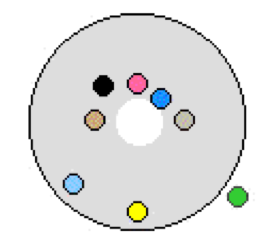
\includegraphics{figures/babble.png}
	\caption{Screenshot of Babble, showing high activity users (in the center) and lower activity users (around the edges), from \citep{Erickson:2003td}.}
	\label{fig:proxy-babble}
\end{marginfigure}

Although Erickson and Kellogg are particularly concerned with what is made visible and what is kept private (the difference between, in their terms, \emph{transparency} and \emph{translucence}), this is a point of divergence between our work. Although I agree with their analysis of the value of considering what actions should be made visible and what should be concealed, it is not a main focus of my analysis. In my work, reading is essentially always invisible and any other action is visible. This is partially a response to their suggestion that it is ``important that participants were aware of the others' awareness of [the properties of the system]'' \citep{Erickson:2003td}. This fits nicely with \citet{Brennan:1991wk}'s presentation of grounding. Simply being told something by someone is not enough for the conversation to move on - you must accept that presentation of information, and that acceptance needs to be accepted by the original presenter. In this way, grounding plays a role not just in communication itself, but in how we communicate information about who we are and what we're doing through actions in the system. 

This finding also suggests that if you don't know which actions are public and which are private, it diminishes the value of translucence as a design strategy. In their work, they tend to rely on physical metaphors to communicate the visibility properties of a system. This is a sensible strategy, but I feel this limits the kinds of experiences we can craft. In my work I tend towards not including invisible actions and instead create completely transparent spaces with carefully selected actions that are worth making visible. This is possible partly because the group sizes in my work are smaller than in the main examples they propose, and it's feasible to show all actions without it being overwhelming. 

\begin{marginfigure}
	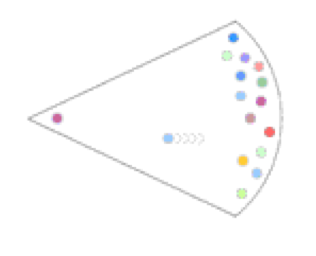
\includegraphics{figures/lecture.png}
	\caption{Screenshot of the lecture proxy, showing the speaker on the left, students on the right, and an interrupting student moving towards the left, from \citep{Erickson:2003td}.}
	\label{fig:proxy-lecture}
\end{marginfigure}

They share a number of specific design findings that complement some of my experiences designing similar systems. They describe three approaches to visualizing activity: realist, mimetic, and abstract. \citep{Erickson:2003td}. I share their interest in abstracted representations, although for different reasons. They argue that realist and mimetic approaches face ``substantial pragmatic barriers (e.g. expense, infrastructure, support)''. In the years since this work was originally done (and well before; one might reasonably argue that \emph{ClearBoard} \citep{Ishii:1992bq} represents an elegant realist approach), many of those pragmatic barriers have fallen. We've seen large-scale virtual worlds (like \emph{Second Life}) that used mimetic approaches and wide adoption of video conferencing which uses realistic representations. Instead, we argue that abstract representations are simply more flexible and better, even given the option of realistic or mimetic approaches.


My work goes into greater depth than Kellogg and Erickson's does on the issue of ``public not personal'' displays. While we agree that it is critical that each person's display doesn't deviate in the kinds of information it represents, in my work these displays are not monolithic---they are not the only venue for interaction between people. Furthermore, displays in my work are most often themselves public, which reinforces the grounding effect. Indeed, that is the most significant deviation between our work. In all of the social proxy work, the proxy is the primary communication medium; in my work, my systems coexist with another primary communication channel, and rarely have any knowledge about the contents of that channel. Public displays also exacerbate issues of attention, which tend not to be major issues for work in the social proxy space (as shown in Table \ref{tab:related-work}). 

% put in a bunch of figures here of the social proxies they designed.



\begin{marginfigure}
	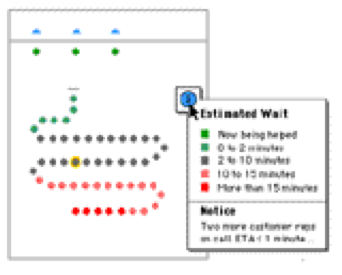
\includegraphics{figures/queue.png}
	\caption{Screenshot of the queue proxy, from \citep{Erickson:2003td}.}
	\label{fig:proxy-queue}
\end{marginfigure}

The other major distinction is in the use of metaphor and display techniques. Erickson and Kellogg box themselves in by limiting their representations to ``a relatively large geometric shape with an inside and an outside and sometimes other features that represent the online situation or context'' \citep{Erickson:2003td} with ``small colored dots'' to represent individual users (similar to \citep{Viegas:1999kv}, minus the direct agency). These design strategies are illustrated in figures \ref{fig:proxy-babble} and \ref{fig:proxy-lecture}. Furthermore, they argue that the best way to represent information is through the use of ``relative movement'' of the user-dots in a way that has ``metaphoric correspondence to the position and movement of people's bodies in face-to-face analogs of the online situation.'' \citep{Erickson:2003td} As I hope my work shows, these limits are not at all necessary to create spaces of meaningful action that facilitate grounded communication and collaboration. Specifically, the need for relying on face-to-face analogs is not a helpful constraint. Instead, my work seeks to create spaces that are easily understood and provide contexts for meaningful action without relying on existing face-to-face metaphors.



\subsection{Channels}

\begin{marginfigure}
	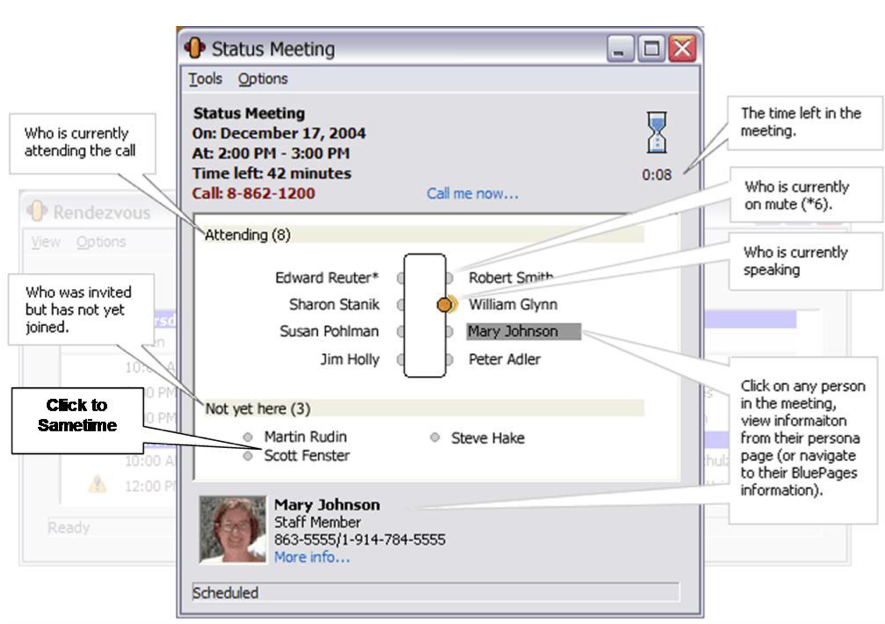
\includegraphics{figures/kellog_social_proxies.png}
	\caption{Screenshot of a meeting-room social proxy for promoting a sense of awareness of other meeting participants, from \citep{kellogg_leveraging_2006}.}
	\label{fig:social-proxies}
\end{marginfigure}

The primary focus of my work is on designing systems that add new communication channels and understanding how those channels operate in contrast to existing channels. In this section, I will present related work that addresses some of these questions.

\begin{marginfigure}
	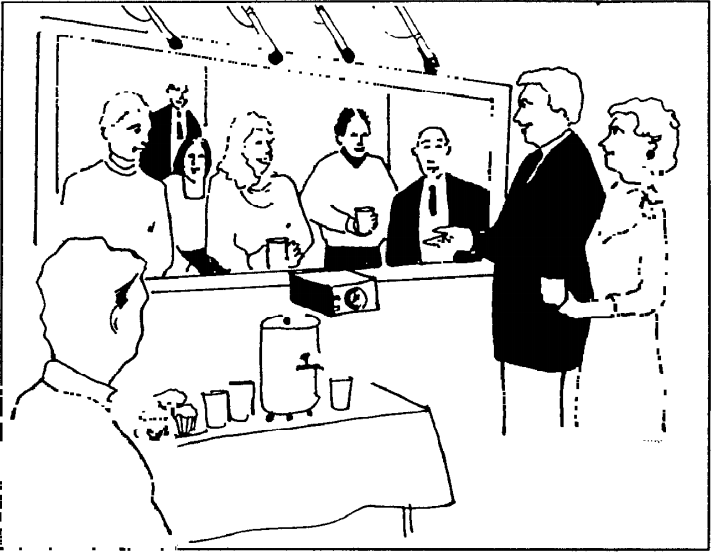
\includegraphics{figures/videowindow.png}
	\caption{Diagram of the VideoWindow scenario for connecting two work-place social spaces, from \citep{Fish:1990fn}}
	\label{fig:videowindow}
\end{marginfigure}

The work most directly related to these questions comes from research into so-called ``backchannels'' in presentation and classroom settings. \citet{Yardi:2006uk} describes how a chat-based backchannel operates over a semester in a classroom, \citet{mccarthy_digital_2004} describe a similar approach at a conference. Backchannels can also be considered a potential part of non-event-oriented contexts too, like long-term co-working among small groups. \citep{Huang:2003ef} Backchannels are not just focused on co-located groups, however, and \citet{kellogg_leveraging_2006} (among others, e.g.  \citep{Yankelovich:2005bx}) has addressed how text and audio backchannels can coexist in distributed contexts. Although past work has addressed in general terms the different ways people use backchannels, it has not sufficiently explained the complicated issues around channel selection, attention, distraction, and identity. Furthermore, in my work I try to move beyond just adding new text or audio channels by adding other kinds of non-verbal actions. In terms of my research themes, past work on backchannels has largely focused on characterizing use patterns, with some discussion of attention. More recent work, like \citep{Bergstrom:wl}, shares an interest in how we can construct actions and how shared displays can be used to help ground the interaction.

\begin{marginfigure}
	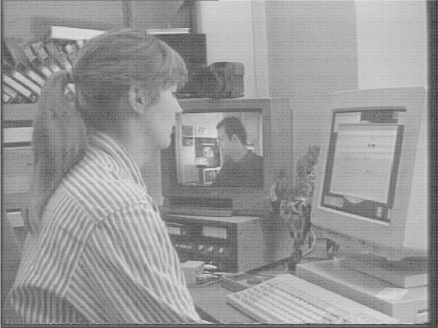
\includegraphics{figures/CRUISER.png}
	\caption{Photo of a CRUISER station installed in an office, from \citep{Fish:1992vz}.}
	\label{fig:cruiser}
\end{marginfigure}

\begin{marginfigure}
	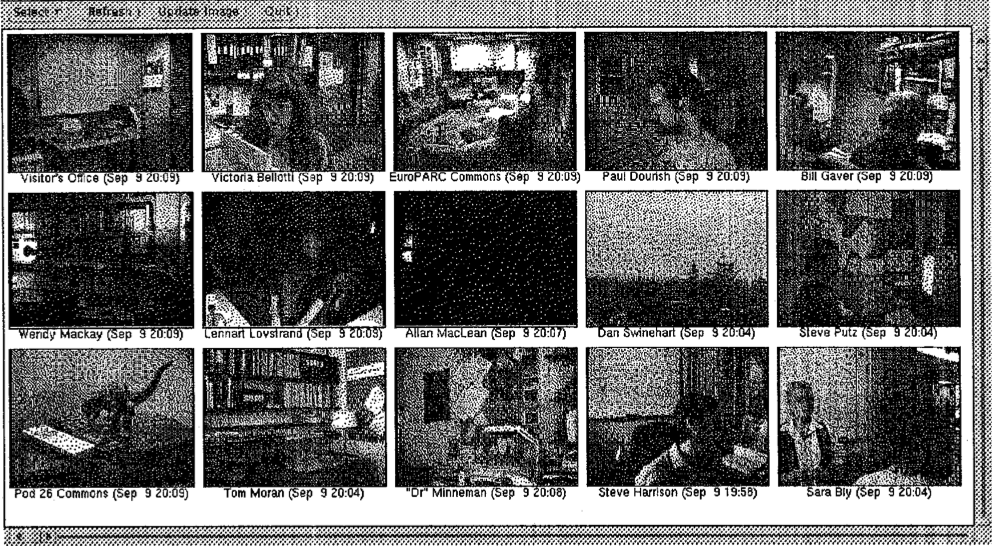
\includegraphics{figures/portholes.png}
	\caption{Screenshot of the Portholes interface, showing periodic stills from a wide range of environmental cameras in an office environment, from \citep{Dourish:1992fu}.}
	\label{fig:portholes}
\end{marginfigure}


Much of the work on creating shared media spaces, driven by experiments at PARC in the late 1980's and early 1990's is salient to my work. Although in some cases this work focused on creating new primary channels, researchers quickly became attuned to problems of privacy and attention because such systems always co-exist with face-to-face communication, in much the same way they do in systems I design. The earliest work at PARC \citep{Olson:1991vz} focused on creating flexible video connections between offices and conference rooms. Subsequent work focused less on a phone-call-like model where connections are created and ended and shifted towards creating spaces with different affordances. Sometimes these involved connecting multiple individuals together, as in CAVECAT \citep{Mantei:1991ww}; other times researchers focused on creating long term persistent video connections in common areas of distributed research groups in the VideoWindow \citep{Fish:1990fn} project. 


Over time, attention shifted more towards a taking advantage of the possibilities to do more than just create ``being there'' experiences. Some researchers experimented with audio-only spaces \citep{Hindus:1996cn}, finding that video was not required to create a sense of connection and space for users, but that the properties of audio did require audio-specific etiquette and coping strategies for the system to be useful. iCom represented a particularly rich design perspective on connecting spaces  \citep{Agamanolis:2003wc}, recognizing that awareness need not be limited to visual awareness, but can extend to information awareness which can be productively embedded in a media space. This embodies the ``beyond being there'' model best of all the work in this research stream: not just trying to create a transparent window between remote spaces, but making something better than a window could be. Furthermore, these projects also focus more on issues of attention, because they are not necessarily always the primary interaction venue for their users. 

% \begin{marginfigure}
% 	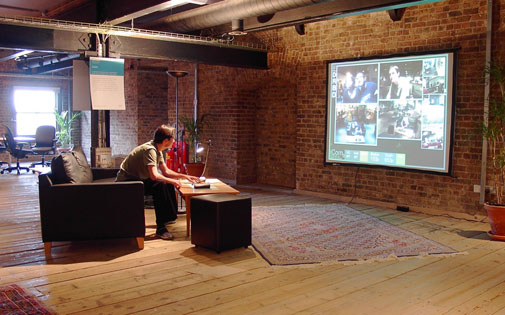
\includegraphics{figures/icom.jpg}
% 	\caption{Photo of one end of an iCom connection, showing multiple video streams and metadata along the bottom of the screen, from \citep{Agamanolis:2003wc}.}
% 	\label{fig:icom}
% \end{marginfigure}


\begin{marginfigure}
	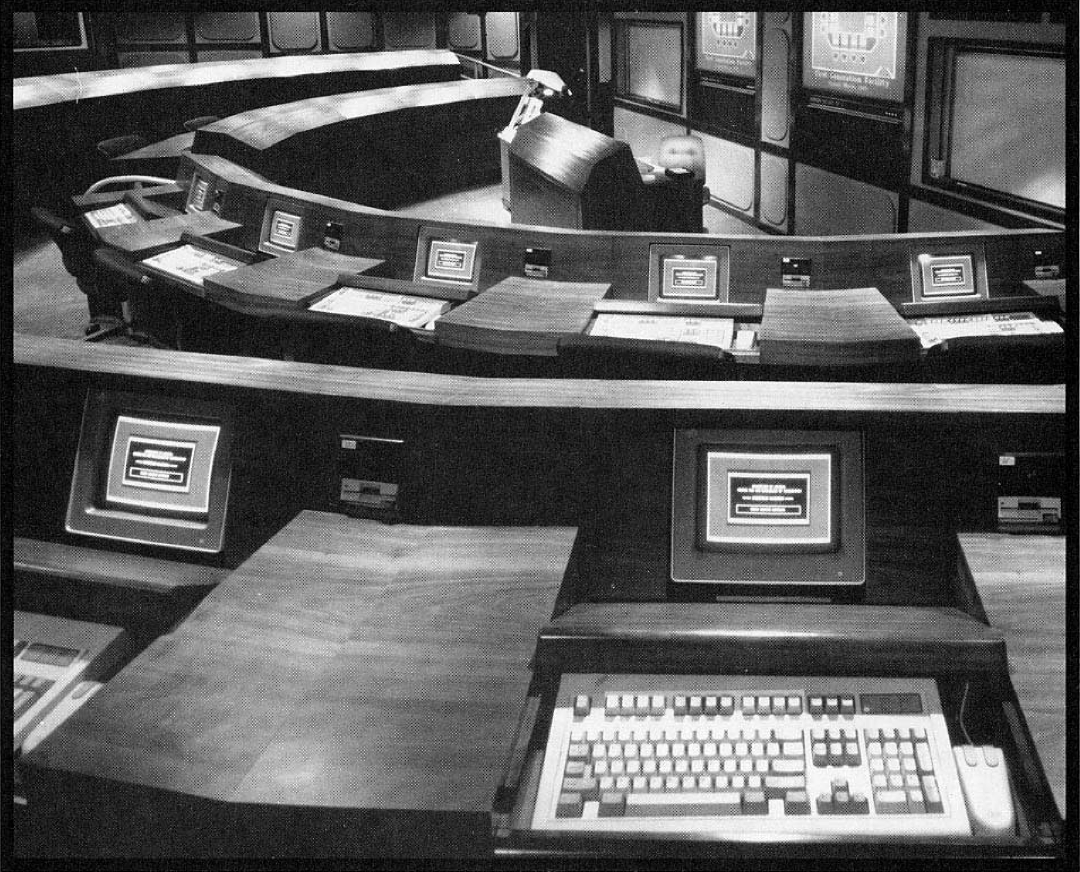
\includegraphics{figures/nunamaker_gdss.png}
	\caption{Photo of a GDSS space, from \citep{nunamaker_electronic_1991}.}
	\label{fig:gdss}
\end{marginfigure}


% also cite karrie's 
% (For subsequent, more artistically inclined approaches to this design space, see Karrie's blah blah, get a nice figure in here for that.)


Serendipity also evolved as an important part of sharing an office environment that was not present with most media space systems. Portholes \citep{Dourish:1992fu} addressed this explicitly by giving people a broader view of remote spaces instead of focusing just on main channel interactions. While my work is not concerned with serendipity, this kind of visual side channel carries important awareness information in much the same way that the side channels in my systems add important contextual information to an interaction. CRUISER \citep{Fish:1992vz} offered non-verbal ways to signal a desire to emulate some of the office hallway etiquette for signaling a desire to drop in and chat informally, without the explicitness of placing a call. The addition of moves like ``cruise'', ``glance'', and ``visit'' are similar in approach to the non-verbal actions at the core of my work like voting in \emph{backchan.nl}, promoting ideas in \emph{Tin Can Classroom}, or moving around the field in \emph{Information Spaces}. 

Early media space researchers proposed a distinction between ``formal'' systems from ``informal'' systems. \citep{Olson:1991vz} While most of the work discussed here (and much of my own work) tends towards the informal side of that continuum, there are some formal elements in my work. This formality manifests most strongly in Group Decision Support Systems research. These systems (exemplified by the work of Nunamaker \citep{nunamaker_electronic_1991}) provide prescriptive systems to support particular brainstorming, decision making, outlining, and voting schemes or policies. In the typical GDSS configuration, each participant has their own computer and interacts with shared structured data in some way, like submitting a new idea or voting on a proposal. In systems like this, the assumption is that having a structured display will ground otherwise informal processes by forcing participants to use the actions the system provides as a set of legitimate conversational moves. Although I tend towards informal systems in my work, the work in this space nonetheless has much to teach us about grounding and actions. 

The lack of consistent results in comparative work in this area \citep{Dennis:1988ww} illustrates the importance of focused design analysis to contextualize findings; it is not useful to view all brainstorming systems as equivalent and comparable in analysis, and I hope that my work will illustrate how the subtleties in interface and approach can have big impacts on outcomes that help explain some of the contradictory results in past GDSS work. Work in this space also raises serious questions related to attention that their work largely fails to address. In fact, in many situations they advocate for largely shutting down pre-existing primary communication channels to focus on the structured, mediated alternative.

Although somewhat rare in the literature, there are a handful of projects that directly address the kinds of hybrid spaces that I seek to create. \emph{Cognoter} \citep{Tatar:1991jq} addresses this design space most clearly. Like my work, \emph{Cognoter} created a hybrid space for very small groups (two to five people) that had both personal and public displays where users could create items and spatially arrange them like on a whiteboard. Textual items can be arranged on a users' display and that arrangement is mirrored on all other users' personal displays. The authors characterize \emph{Cognoter}'s model of creating shared text elements as representing a ``parcel-post'' as opposed to an ``interactive'' conversational model. Instead of embodying a present/accept process (as described by \citep{Clark:1989uc}), they describe their process as being more like literary communication (like email) where the writer tries to make sure ``that the addressees \emph{should have been able} to understand his meaning in the last utterance'' (emphasis mine). This is in contrast to face-to-face interaction, where we can interactively ascertain the extent to which we are being understood (and repair mistakes) before moving on. The authors describe \emph{Cognoter}'s failure to be used effectively by its users as (in part) a conflict between the interactive mode of face-to-face communication and the parcel-post model in \emph{Cognoter}. The \emph{Thoughtswap} project \citep{DickeyKurdziolek:2010wt} also shares my goal in creating hybrid spaces, but like \emph{Cognoter}, the mediated space is used serially with the face-to-face space, while I am interested in creating spaces for legitimate simultaneous performances in mediated and non-mediated spaces. This suggests a major hurdle for my work: can you create systems that use a parcel-post model yet still integrate fluidly with the interactive face-to-face model? \emph{Cognoter} and \emph{Thoughtswap} suggest this is hard, but I will show throughout my work how these barriers can be overcome and suggest ways to explain \emph{Cognoter}'s negative findings.

% go hunting for a desanctis and/or poole piece that's not focusing on AST specifically? also can hit berg if we want, but it feels like a bit of a distraction at the moment.

%, they also produced a nice taxonomy of the kinds of tools that would be useful for distributed collaborative groups: synchronous versus asynchronous communication and open processes versus focused processes, a distinction 


% there's a funny note in the portland paper about how they want to shift away from meeting augmentation to async and task coordination. Funny how times change.

% now summarize. 


% going to want to bring up media equation or whatever that book is called. Cliff Nass. 




% thundewire is just audio, basically a single-channel mumble. not so much about results as describing practices that evolved. 
% portholes is ambient awareness about remote places, not live interaction. cut it?
% videowindow is just like hole in space - audio/video fixed in space

% also mention virtual world stuff? MASSIVE might be worth a quick ref

% "shared media systems"

% - video projects like thunderwire + portholes
% - videowindow


% organize the work in this space 
% projects to talk about:
% - voiceloops
% - backchannel literature
% - social proxies
% - mention conferencing apps
% - Nunamaker
% - zephyr?


% \subsection{Theoretical Perspectives}
% thinking about leaving this out

% stuff from cscw paper:
% systems for reflection
% - second messenger
% - "social mirror" (Karahalios) also bergstrom
% - Meeting Mediator
% 
% systems adding new channels
% - (all the backchan literature: yardi, mccarthy, huang, kellog, yankelovich)
% - do a section on nunameker's work and why it's weird
% - 

% - we'll want to at the very least nod to thinks like voiceloops, and all the audio/video stuff like portholes and thunderwire and that kind of thing. farm my generals reading for that part.
%


% theoretical perspectives
% - practice lens?
% - ethnomethodology? 
% - re-farm wanda's reading list to see what else I can pull from there.

%
% We'll need to do a little organization here. Obviously, farm the references from the Tin Can Edu CSCW paper + backchan.nl paper. We'll need more, ofc, but it's a start. I suspect there will be some ways to separate out systems that allow communication versus those that simply reflect on a main channel. Maybe it's about whether the system itself is a single channel, multi channel, main channel or side channel? 

% write a methodological section here about why it's useful to study this with design work

\subsection{Reflection}

\begin{marginfigure}
	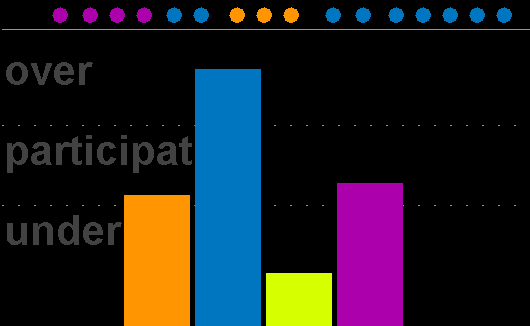
\includegraphics{figures/second-messenger.png}
	\caption{Screenshot of a Second Messenger participation bar-chart, from \citep{DiMicco:2007ie}.}
	\label{fig:second-messenger}
\end{marginfigure}

% \begin{marginfigure}
% 	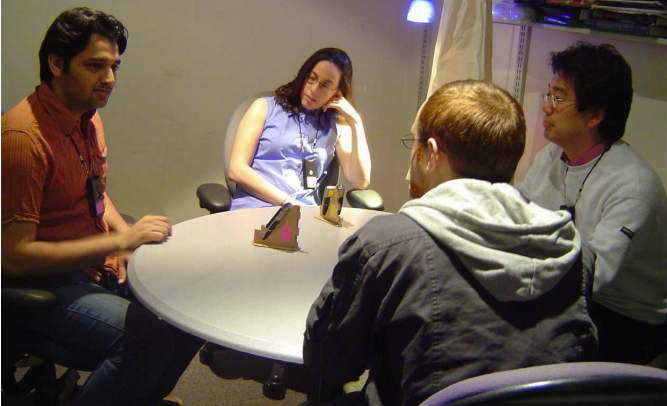
\includegraphics{figures/meeting_mediator.png}
% 	\caption{Meeting mediator.}
% 	\label{fig:meeting-mediator}
% \end{marginfigure}




Understanding how we present ourselves to others has been a topic of sociological inquiry for quite some time. Although many of the insights of scholars like \citet{goffman_presentation_1959} about how we communicate and interpret information about who we are and how we want to be treated are still relevant, the information that is available about people has changed substantially. In some of the examples in this section, designers have added some new bit of information about people to a face to face discussion; in others, we don't have any of the traditional information we would get from being face to face with someone and rely on new types of signals (like the non-verbal actions I propose) to create a sense of people around us. Part of what sets mediated communication apart is the ability to accumulate behavioral histories and represent and reflect those histories to ourselves and others. The work in this space is not as closely connected to my main research themes, but I include it here primarily because it has served as a source of design inspiration. 


\begin{marginfigure}
	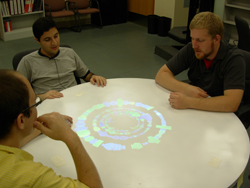
\includegraphics{figures/conversation_clock.png}
	\caption{Photo of Conversation Clock in use, showing relative participation histories from each conversation participant, from \citep{Bergstrom:2007je}.}
	\label{fig:conversation-clock}
\end{marginfigure}

My work is substantially inspired by the work of \citet{DiMicco:2007ie} on the \emph{Second Messenger} project. In this project, participants in a group discussion were presented with a constantly-updating bar-chart visualization representing the relative amount of time they had talked during the discussion. They found that while people who over-participated without a visualization tended to moderate their participation when the visualization was present, people with low participation did not participate more just because others were participating less. \emph{Meeting Mediator} \citep{Kim:2008ip} took a similar approach, but focused on situations where groups of two people could see each other and had to interact with another group of two people who they could only hear. Using a different visualization, Kim et al. found that groups were more interactive with the system than without, although there was not a correlation with group performance. 

\begin{marginfigure}
	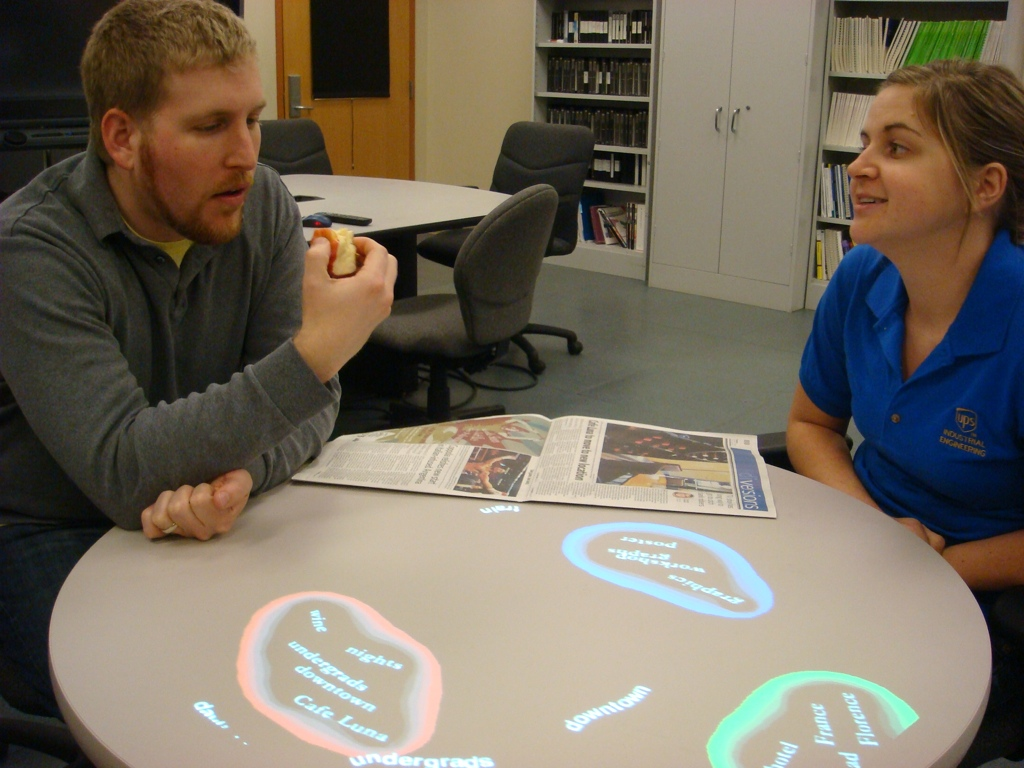
\includegraphics{figures/conversation_clusters.jpg}
	\caption{Photo of \emph{Conversation Clusters}, detecting audio themes and displaying them in visual clusters on the table-top display, from  \citep{Bergstrom:2009fe}.}
	\label{fig:conversation-clusters}
\end{marginfigure}


Bergstrom has done a series of projects that adopt a similar design strategy. \emph{Conversation Clusters} \citep{Bergstrom:2009fe} pulls topics from an audio conversation and presents them in clusters on a table-top display. \emph{Conversation Clock} \citep{Bergstrom:2007je}, like \emph{Second Messenger} and \emph{Meeting Mediator}, visualizes conversation participation, but uses a timeline metaphor instead of a aggregative metaphor. \emph{Conversation Votes} \citep{Bergstrom:2009ej} lets uses discreetly vote about the progress of a discussion, and displays anonymous votes on a table-based display. \citet{Karahalios:hu} describes this design space as ``social mirrors''. 

\begin{marginfigure}
	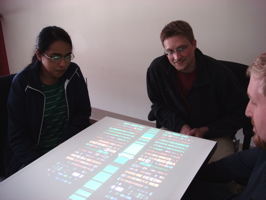
\includegraphics{figures/conversation_votes.jpg}
	\caption{Photo of \emph{Conversation Votes}, showing voting history among conversation participants on the table-top display, from \citep{Bergstrom:2009ej}.}
	\label{fig:conversation-votes}
\end{marginfigure}


% sneak in a \citep{visiphone} here?


% MATT TODO FIX THE MIDDLE OF THIS PARAGRAPH IT'S AWFUL
These are all examples of the accumulate and reflect design strategy, where the system tracks some aspect of behavior: spoken participation in the case of \emph{Second Messenger} and \emph{Meeting Mediator}, discussion topics and group attitudes in the case of Bergstrom's work. 

%The systems then present that information back to the individual or group with the intention that to reflect on and adjust their behavior. Furthermore, all of these projects have an element of grounding to them. By presenting this social information on a shared display (as in my work), it is made salient to the discussion in a way that private displays cannot.

% cite things like last.fm, goodreads, etc in this space?


% \subsection{Identity}

% maybe this whole section is dumb.
% how often do I really deal with this? It's clearly part of the second life work, but not at all part of backchannl, and only a little a part of the Tin Can series. Erm. Move on for now and double back. 

% Many other projects have focused on how peoples' identities are presented. In most of these pieces, there is no face-to-face element, which drives the researcher's interest in developing compelling alternative options that can richly communicate who someone is in a mediated space. Many informal and practical options are in common use; displaying an icon or image chosen by someone and a pseudonym to represent themselves is a widely used design strategy in social applications throughout the internet. These spaces for self expression are frequently augmented by systems that aggregate someone's behavior in that space. This is much like the reflection techniques, but are usually summarizing events beyond any single person's experience. The community site StackOverflow \citep{stack_overflow} provides a particularly rich example of this strategy.

% screenshot a wow forum, stackoverflow, 

% These techniques feel thin compared to the richness of face-to-face interaction, and researchers have developed a number of alternative approaches. Donath's work on data portraiture in a variety of 



% link to things like Ros' work in terms of augmenting face to face interaction with extra information? Or go back to steve mann's cyborg stuff?

% need a paragraph here that's more about the identity side of things. not sure what that will be. chat circles, perhaps? talking in circles? (whichever one had that intersting voting shapes thing)

% how to fit in social proxies and social translucense



% Other potential bits we could fill in here...
% We could spend some time with social translucense
% We could look at non-vebal actions as a space
%	start with Greenbergs stuff, but really look all over for groupware/collaborative tools that had some action to them. Will find some of that in the CVE literature, which might be easy to find
% I don't talk at all about theory stuff here. Could do the spiel about shared displays and grounding, but I'm not sure how critical that is going to be ultimately.
%
%
%  One other strategy is to think about the three research themes: grounding, non-verbal actions, and attention, and go on a hunt for good literature about each of those. 


\subsection{Meeting Structure}

Any system designed to support interaction makes a number of implicit assumptions about the nature of the social process it's trying to support. This is true across design domains. For instance, calendaring systems often assume that the important aspects of someone's work life can be captured in meetings. Meetings have a time, a place, and other meeting participants. Certainly, this describes some kinds of work life, but plenty of other jobs don't fit with that metaphorical structure. Imagine a car repair shop; a system to support that sort of work environment would necessarily be concerned with specific tasks that need to be done and which people in the shop were going to do them. A meeting organization system would not be as appropriate for managing that environment. Of course, over time systems influence people's behavior in such a way that it makes it hard to distinguish between the implicit assumptions about how people would use the system and how their behavior has adjusted to best make use of the systems they have available. 

Meetings are rich social experiences that are composed of a variety of deeply interconnected components. I turn to \citet{McGrath:1984un}'s theoretical framework as a good starting place for understanding the diversity of factors that influence a group's process. McGrath describes groups as ``task performance systems'', recognizing the critical extent to which tasks characterize a group's interaction, along with the group composition, the properties of the environment, and properties of the individual. He identifies eight types of tasks: planning, creativity, intellective, decision-making, cognitive conflict, mixed-motive, competitive, and performance. In this chapter we are primarily concerned with decision-making tasks.

Various structures for organizing decision-making have been proposed. One interesting structure is IBIS \citep{Kunz:1970wo}, which classifies the structure of arguments in design meetings. In their model, a discussion has Issues (e.g. ``Users aren't using this feature as much as we thought they would''), Positions (``We should include the feature in our tutorial'') and Arguments (``Not many users are following the tutorial either, we need another way to promote this feature.'') These objects are linked by different relationships, like ``supports'', ``objects-to'', ``responds-to'' or ``specializes''. This creates an abstract argument network that organizes the discussion around concrete issues. \citet{Conklin:1988fr} describe a computer-supported system that uses this structure for both synchronous and asynchronous discussions. This basic approach of modeling a particular task network in a formal way is shared by many Group Decision Support Systems of which \citet{nunamaker_electronic_1991} is a nice overview.

In McGrath's terms, though, systems like gIBIS (and many of the systems described in the GDSS literature) are not strictly addressing one task. They're nominally about making decisions, but a group using gIBIS is also sometimes trying to solve intellective tasks (e.g. solving questions with a single right answer), generative tasks, and perhaps resolving conflict tasks. The precise mix of these tasks varies in each group's process, which creates a significant diversity in system designs. Structures that assume a particular task profile are unlikely to be effective when applied to another task profile.

Task profiles are one example of a formalizing instinct to organize and abstract certain features of human practice in a way that can help us both better understand those practices or (in the case of designers) design tools that support those practices. Not only is it a question of useful or accurate abstractions, it is also a tension between the right amount of structure and too much structure. A model like IBIS or Roberts' Rules of Order \citep{RobertIII:2000tq} is relatively heavy amount of structure. In contrast, process models like nominal group technique \citep{Bartunek:1984cq} operate at an even higher level of abstraction. In general, my instincts lean towards less formality rather than more, but that reflects the sorts of practices I'm creating tools for more than a real argument for either strategy. Regardless of how one decides to abstract, there is still a complex relationship between the selected formalism and the practice it is either modeling or seeking to promote. \citet{Berg:1997bs} describes this interplay this way:

\begin{quotation}
By offering abstracted models of the work and/or by processing input into output, formal tools are attributed central roles in organizing the work within the workplace.
\end{quotation}

Berg organizes the camps on this issue into two main discourses: naive formalists who believe that formal models are necessary for rational or scientific decision-making or work. In contrast, one can make the argument that the richness of the empirical world defies our ability to always reduce it to formal models. This argument has a political angle to it, as well, arguing that (as Berg describes it) formal tools will ``inevitably function in a rigid, impoverished way, thus de-skilling and dehumanizing the work of those who are caught in its cold, instrumental rationality.'' These are both extreme views and not widely held at this point. Berg characterizes the distinction between the formal tool and the human practice as being like the distinction between the map and the terrain it describes. Maps are a way of abstracting and describing terrain, while also influencing the ways that people understand and develop that terrain. They are necessarily tightly interrelated.

Although Berg is primarily interested in building theoretical tools for better understanding practices at the boundary between formal tools and human practices, this perspective is valuable too for designers. Formal model building is a critical step in designing any sort of software system. Indeed, designing abstract representational models for data is a core part of any software design process. \sidenote{\citet{Hughes:tv} is a clever (if somewhat inaccessible to non-database engineers) analysis of the challenges representing human marriage practices in a database. It illustrates, too, the built in biases of computational systems towards certain sorts of abstractions.} In this mode we are faced with the problems of building the map from scratch, and trying to understand the relationship between the sort of map we build and the terrain it describes. Furthermore as researchers we frequently have our own agendas and are trying to describe future terrains that may not exist yet. Put another way, maps are sometimes guides to exciting new terrain, not just describing a certain perspective on existing terrain. This is more precisely the sort of work that I do.

As I describe each of my projects, I will attempt to describe the sorts of existing practices it seeks to support as well as the sorts of practices it aims to encourage through a certain sort of formalization. 







% Another model with a task profile more focused on resolving conflicting viewpoints is the Public Conversations Project \citep{PublicConversations:ta} uses a system for having dialog about controversial issues (e.g. Israel/Palestine, reproductive rights, etc.) that focuses on the context and structure of the meeting. These meetings are intentionally not about reaching consensus, but instead about building understanding, which makes an argument-based structure like IBIS inappropriate.
% 
% 
% Part of what's exciting about working in virtual worlds is that the basic rules of a space don't preclude lots of different kinds of interfaces being built within it. The system I propose in this chapter is a simple model (neither IBIS or the PCP models) that is appropriate for only certain kinds of meetings. I imagine it as being one of eventually a set of spaces designed to work for specific situations. Just as a company might choose to use IBIS for some of its meetings, a meeting moderator in a virtual world can choose to use this space or some other virtual space for their meeting depending on whether or not their needs and the structure of their interactions are a good fit for the space.
